\chapter{MARCO TEORICO}

%%%%%%%%%%%%%%%%%%%%%%%%%%%%%%%%%%%%%%%%%%%%%   PROCESO KDD   %%%%%%%%%%%%%%%%%%%%%%%%%%%%%%%%%%%%%%%%%%%%%%%%%
\section{El Proceso de Descubrimiento de Conocimiento en Bases de Datos - DCBD}
El proceso de DCBD es el proceso que utiliza m\'etodos de miner\'ia de datos (algoritmos)
para extraer
(identificar) patrones que evaluados e interpretados, de acuerdo a las especificaciones
de medidas y umbrales,
usando una base de datos con alguna selecci\'on, preprocesamiento, muestreo y
transformaci\'on, se obtiene lo que
se piensa es conocimiento \cite{9}.\\
\\
El proceso de DCBD es interactivo e iterativo, involucra numerosos pasos con la
intervenci\'on del usuario en la
toma de muchas decisiones y se resumen en las siguientes etapas:

\begin{itemize}
\item Selecci\'on.
\item Preprocesamiento / Data cleaning.
\item Transformaci\'on / Reducci\'on.
\item Miner\'ia de Datos (Data Mining).
\item Interpretaci\'on / evaluaci\'on.
\end{itemize}

%%%%%%%%%%%%%%%%%%%%%%%%%%%%% Integraci\'on herramientas DCBD con SGBD %%%%%%%%%%%%%%%%%%%%%%%%%%%%%%%%%%%%%%%%%
\section{Arquitecturas de Integraci\'on de las Herra\-mientas DCBD con un SGBD}
Las arquitecturas de integraci\'on de las herramientas DCBD con un SGBD se pueden ubicar
en una de tres tipos:
herramientas d\'ebilmente acopladas, medianamente acopladas y fuertemente acopladas con
un SGBD \cite{30}.\\
\\
Una arquitectura es d\'ebilmente acoplada cuando los algoritmos de Miner\'ia de Datos y
dem\'as componentes se
encuentran en una capa externa al SGBD, por fuera del n\'ucleo y su integraci\'on con
este se hace a partir de una
interfaz \cite{30}.\\
\\
Una arquitectura es medianamente acoplada cuando ciertas tareas y algoritmos de
descubrimiento de patrones se
encuentran formando parte del SGBD mediante procedimientos almacenados o funciones
definidas por el usuario
\cite{30}.\\
\\
Una arquitectura es fuertemente acoplada cuando la totalidad de las tareas y algoritmos
de descubrimiento de
patrones forman parte del SGBD como una operaci\'on primitiva, dot\'andolo de las
capacidades de descubrimiento de
conocimiento y posibilit\'andolo para desarrollar aplicaciones de este tipo \cite{30}.\\
\\
Por otra parte, de acuerdo a las tareas que desarrollen, las herramientas DCBD se
clasifican en tres grupos:
herramientas gen\'ericas de tareas senci\-llas, herramientas gen\'ericas de tareas
m\'ultiples y herramientas de
dominio espec\'ifico.\\
\\
Las Herramientas gen\'ericas de tareas sencillas principalmente soportan solamente la
etapa de miner\'ia de datos
en el proceso de DCBD y requieren un pre y un post procesamiento de los datos. El usuario
final de estas
herramientas es t\'ipicamente un consultor o un desarrollador quien podr\'ia integrarlas
con otros m\'odulos como
parte de una completa aplicaci\'on.\\
\\
Las Herramientas gen\'ericas de tareas m\'ultiples realizan una variedad de ta\-reas de
descubrimiento,
t\'ipicamente combinando clasificaci\'on, asociaci\'on, visualizaci\'on, clustering,
entre otros. Soportan
diferentes etapas del proceso de DCBD. El usuario final de estas herramientas es un
analista quien entiende la
manipulaci\'on de los datos.\\
\\
Finalmente, las Herramientas de dominio espec\'ifico, soportan descubrimiento solamente
en un dominio espec\'ifico
y hablan el lenguaje del usuario final, quien necesita conocer muy poco sobre el proceso
de an\'alisis.
\newpage
\section{Implementaci\'on de  Herramientas DCBD d\'ebilmente acopladas con un SGBD}
\begin{figure}[h]
   \centering
   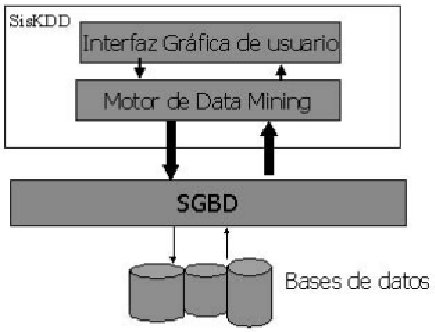
\includegraphics[width=10cm,height=8cm]{imgsMteorico/arquitectura.jpg}
   \caption{Arquitectura DCBD d\'ebilmente acoplada}
   \label{fig1}
\end{figure}

La implementaci\'on de herramientas DCBD d\'ebilmente acopladas con un SGBD se hace a
trav\'es de SQL embebido en
el lenguaje anfitri\'on del motor de miner\'ia de datos \cite{3}.  Los datos residen en
el SGBD y son le\'idos
registro por registro a trav\'es de ODBC, JDBC o de una interfaz  de cursores SQL. La
ventaja de esta arquitectura
es su portabilidad. Sus principales desventajas son la escalabilidad y el rendimiento. El
problema de
escalabilidad consiste en que las herramientas y aplicaciones bajo este tipo de
arquitectura,  cargan todo el
conjunto de datos en memoria, lo que las limita para el manejo de grandes cantidades de
datos. El bajo rendimiento
se debe a que los registros son copiados uno por uno  del espacio de direccionamiento de
la base de datos al
espacio de direccionamiento de la aplicaci\'on de miner\'ia de datos \cite{6,15}  y
estas  operaciones de
entrada/salida,  cuando se manejan grandes vol\'umenes de datos,  son bastante costosas,
a pesar de la
optimizaci\'on de lectura por bloques presente en muchos SGBD (Oracle, DB2, Informix,
PostgreSQL.) donde un bloque
de tuplas puede ser le\'ido al tiempo (figura 1).

%%%%%%%%%%%%%%%%%%%%%%%%%%%%%%%%%%%%%%%%%%%%%%%% ALGORITMOS %%%%%%%%%%%%%%%%%%%%%%%%%%%%%%%%%%%%%%%%%%%%%%%%%%
\section{Algoritmos implementados en TariyKDD}

\subsection{Apriori}
La notaci\'on del algoritmo Apriori \cite{4} es la siguiente:\\

\begin{table}[h]
\caption{Notaci\'on algoritmo Apriori}
\end{table}
\begin{center}
\begin{tabular}{|p{40mm}|p{40mm}|}\hline
\textbf{$k$-itemset} & \textbf{Un itemset con $k$ items}\\ \hline
$L_{k}$              & Conjunto de itemsets frecuentes $k$ (Aquellos con soporte m\'inimo).\\ \hline
$C_{k}$              & Conjunto de itemsets candidatos $k$ (Itemstes potencialmente frecuentes)\\ \hline
\end{tabular}
\end{center}


A continuaci\'on se muestra el algoritmo Apriori:\\ \\
\begin{footnotesize}
\noindent 		$L_{1} =$ \{Conjunto de itemsets frecuentes 1 \}\\
	  		for ( $k=2;\ \ L_{k-1}\neq0;\ \  k++$  ) do begin\\
\indent   		$C_{k}=$ apriori-gen$(L_{k-1})$ // Nuevos candidatos\\
\indent 		forall $transacciones\ \ t\in D$ do begin\\
\indent\indent 			$C_{t}=$ subconjunto $(C_{k}, t);$ // Candidatos en t\\
\indent\indent 			forall $candidatos\ \ c \in C_{t}$ do\\
\indent\indent\indent 			$c.cont++;$\\
\indent 			end\\
\indent 		$L_{k}=$ \{ $c \in C_{k} | c.count \geq minsup$ \}\\
			end
			Answer $\cup_{k} L_{k}$\\
\end{footnotesize}

La primera pasada del algoritmo cuenta las ocurrencias de los items en todo el conjunto de datos para determinar
los itemsets frecuentes 1. Los subsecuentes pasos del algoritmo son basicamente dos, primero, los itemsets
frecuentes $L_{k-1}$ encontrados en la pasada $(k-1)$ son usados para generar los itemsets candidatos $C_{k}$,
usando la funci\'on apriori-gen descrita en la siguiente subsecci\'on. Y segundo se cuenta el soporte de los
itemsets candidatos $C_{k}$ a trav\'es de un nuevo recorrido a la base de datos. Se realiza el mismo proceso
hasta que no se encuentren m\'as itemsets frecuentes.

\subsubsection{Generaci\'on de candidatos en Apriori}
La funci\'on apriori-gen toma como argumento $L_{k-1}$, o sea todos los itemsets frecuentes $(k-1)$. La funci\'on
trabaja de la siguiente manera:\\

\begin{footnotesize}
\noindent 	insert into $C_{k}$\\
	  	select $p.item_{1},\ \ p.item_{2},...,\ \ p.item_{k-1},\ \ q.item_{k-1}$\\
		from $L_{k-1}\ \ p,\ \ L_{k-1}\ \ q$\\
		where $p.item_{1}=q.item_{1},...,\ \ p.item_{k-2}=q.item_{k-2},$\\
\indent			$p.item_{k-1}\<q.item_{k-1};$\\
\end{footnotesize}

A continuaci\'on, en el paso de poda, se borran todos los itemsets $c \in C_{k}$ tal que alg\'un subconjunto
$(k-1)$ de $c$ no este en $L_{k-1}$:\\

\begin{footnotesize}
forall $itemsets\ \ c \in C_{k}$ do\\
\indent forall subconjuntos $(k-1)\ \ s$ de $c$ do\\
\indent\indent if $(s \notin L_{k-1})$ then\\
\indent\indent\indent delete $c$ from $C_{k};$
\end{footnotesize}


\subsection{FPGrowth}
Como se puede ver en \cite{15} la heur\'istica utilizada por Apriori logra buenos resultados, ganados por
(posiblemente) la reducci\'on del tama\~no del conjunto de candidatos. Sin embargo, en situaciones con largos
patrones, soportes demasiado peque\~nos, un algoritmo tipo Apriori podr\'ia sufrir de dos costos no triviales:

\begin{itemize}
\item Es costoso administrar un gran n\'umero de conjuntos candidatos. Por ejemplo, si hay $10^{4}$ Itemsets
Frecuentes, el algoritmo Apriori necesitar\'a generar m\'as de $10^{7}$ Itemsets Candidatos, as\'i como acumular
y probar su ocurrencia. Adem\'as, para descubrir un patr\'on frecuente de tama\~no 100, como
${a_{1},...,a_{100}}$, se debe generar m\'as de $2^{100}$ candidatos en total.
\item Es una tarea demasiado tediosa el tener que repetidamente leer la base de datos para revisar un gran
conjunto de candidatos.
\end{itemize}
El cuello de botella de Apriori es la generaci\'on de candidatos \cite{15}. Este problema es atacado por los
siguientes tres aspectos:\\

Primero, una innovadora y compacta estructura de datos llamada \textit{\'Arbol de Patrones Frecuentes} o 
\textit{FP-tree} por sus siglas en ingles (\textit{Frequent Pattern Tree}), la cual es una estructura que 
almacena informaci\'on crucial y cuantitativa acerca de los patrones frecuentes. \'Unicamente los itemsets
frecuentes 1 tendr\'an nodos en el \'arbol, el cual esta organizado de tal forma que los items m\'as
frecuentes de una transacci\'on tendr\'an mayores oportunidades de compartir nodos en la estructura.\\ \\
Segundo, un m\'etodo de Miner\'ia de patrones crecientes basado en un FP-tree. Este comienza con un patr\'on
frecuente tipo 1 (como patr\'on sufijo inicial), examina sus Patrones Condicionales Base (una ''sub-base de
datos'' que consiste en el conjunto de items frecuentes, que se encuentran en patr\'on sufijo), construye su
FP-tree (condicional) y dentro de este lleva a cabo recursivamente Miner\'ia. El patr\'on creciente es 
conseguido a trav\'es de la concatenaci\'on del patr\'on sufijo con los nuevos generados del FP-tree condicional.
Un itemset frecuente en cualquier transacci\'on siempre se encuentra en una ruta de los \'arboles de Patrones
Frecuentes.\\ \\
Tercero, la t\'ecnica de busqueda empleada en la Miner\'ia esta basada en particionamiento, con el m\'etodo
''divide y venceras''. Esto reduce dramaticamente el tama\~no del Patr\'on Condicional Base generado en el 
siguiente nivel de busqueda, as\'i como el tama\~no de su correspondiente FP-tree. Es m\'as, en vez de buscar
grandes patrones frecuentes, busca otros m\'as peque\~nos y los concatena al sufijo. Todas estas t\'ecnicas 
reducen los costos de busqueda.

\subsubsection{Dise\~no y construcci\'on del \'Arbol de Patrones Frecuentes (FP-tree)}
Sea $I={a_{1},a_{2},...,a_{m}}$ un conjunto de items, y $DB={T_{1},T_{2},...,T_{m}}$ una base de datos de
transacciones, donde $T_{i}(i \in [1...n])$ es una transacci\'on que contiene un conjunto de items en $I$. El
soporte (u ocurrencia) de un patr\'on $A$ o conjunto de items, es el n\'umero de veces que $A$ esta contenida en
$DB$. $A$ es un patr\'on frecuente, si el soporte de $A$ es mayor que el umbral o soporte m\'inimo, $\xi$.

\paragraph{\'Arbol de Patrones Frecuentes}
A trav\'es del siguiente ejemplo se examina como funciona el dise\~no de la estructura de datos para minar con
eficiencia patrones frecuentes.

\subparagraph{Ejemplo 1}
Sea la base de datos de transacciones, cuadro \ref{tid} y $\xi=3$. Una estructura de datos puede ser dise\~nada de
acuerdo a las siguientes observaciones:
\begin{enumerate}
\item Aunque solo los items frecuentes jugar\'an un rol en la Miner\'ia de Patrones Frecuentes, es necesario leer 
la BD para identificar este conjunto de items.
\item Si se almacenan items frecuentes de cada transacci\'on en una estructura compacta, se podr\'ia
evitar el tener que leer repetidamente la BD.
\item Si m\'ultiples transacciones comparten un conjunto id\'entico de items frecuentes, estas pueden ser
fusionadas en una sola, con el n\'umero de ocurrencias como contador.
\item Si dos transacciones comparten un prefijo com\'un, las partes compartidas pueden ser unidas usando una
estructura prefija. Si los items frecuentes son ordenados descendientemente, habr\'a mayor probabilidad de que los
prefijos de las cadenas esten compartidos.
\end{enumerate}

\begin{table}[h]
\caption{Base de Datos de transacciones}
\label{tid}
\end{table}
\begin{center}
\begin{tabular}{|p{25mm}|p{30mm}|p{40mm}|}\hline
\textbf{TID} & \textbf{Items} & \textbf{Items frecuentes (ordenados)}\\ \hline\hline
100 & f,a,c,d,g,i,m,p & f,c,a,m,p\\ \hline
200 & a,b,c,f,l,m,o   & f,c,a,b,m\\ \hline
300 & b,f,h,j,o       & f,b\\ \hline
400 & b,c,k,s,p       & c,b,p\\ \hline
500 & a,f,c,e,l,p,m,n & f,c,a,m,p\\ \hline
\end{tabular}
\end{center}

\begin{figure}[ht]
   \centering
   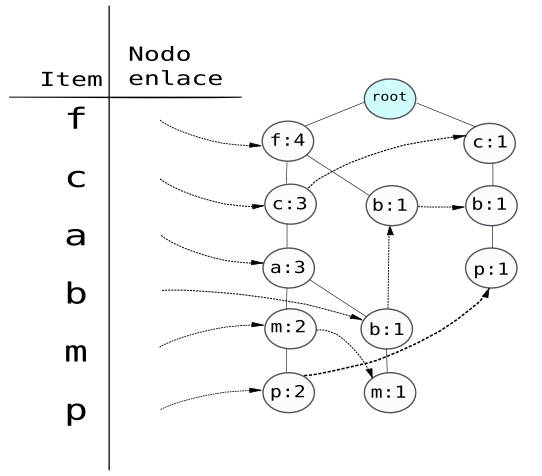
\includegraphics[width=0.6\textwidth]{images/fptree1.png}
   \caption{Tabla de cabeceras y Arbol FP-tree del ejemplo 1}
   \label{fptid}
\end{figure}

\newpage

Con estas observaciones se puede construir un \'Arbol de Patrones Frecuentes de la siguiente forma:\\ \\
Primero, el leer $DB$ genera una lista de items frecuentes, $\{(f:4),(c:4),(a:3),(b:3),(m:3),(p:3)\}$, (el
n\'umero indica el soporte) ordenados descendientemente.\\ \\
Segundo, crear la ra\'iz del \'arbol con un \textit{null}. Al leer la primera 
transacci\'on se construye la primera rama del \'arbol $\{(f:1),(c:1),(a:1),(m:1),(p:1)\}$. Para la segunda 
transacci\'on ya que su lista de items frecuentes $(f,c,a,b,m)$ comparte el prefijo com\'un $(f,c,a)$ con la rama
existente $(f,c,a,m,p)$, el conteo de cada nodo en el \'arbol prefijo es incrementado en 1, dos nuevos nodos son
creados, $(b:1)$ enlazado como hijo de $(a:2)$ y $(m:1)$ enlazado como hijo de $(b:1)$. Para la tercera 
transacci\'on como su lista de frecuentes solamente es $(f,b)$ y el \'unico prefijo compartido es $(f)$, el
soporte de $(f)$ se incrementa en 1, y un nuevo nodo $(b:1)$ es creado y enlazado como hijo de $(f:3)$. La
lectura de la cuarta transacci\'on lleva a la construcci\'on de la segunda rama del \'arbol,
$\{(c:1),(b:1),(p:1)\}$. Para la \'ultima transacci\'on ya que su lista de items frecuentes $(f,c,a,m,p)$ es
identica a la primera, la ruta es compartida, incrementado el conteo de cada nodo en 1.\\ \\
Para facilitar m\'as el funcionamiento del \'arbol una Tabla de Cabeceras es construida, en la cual cada item
apunta a su ocurrencia en el \'arbol. Los nodos con el mismo nombre son enlazados en secuencia y despu\'es de
leer todas las transacciones, se puede ver el \'arbol resultante en la figura \ref{fptid}.\\ \\
Por tanto un \textbf{\'Arbol de Patrones Frecuentes (FP-tree)} es una estructura como se define a
continuaci\'on:\\

\begin{itemize}
\item Consiste de una raiz etiquetada como \textit{null}, un conjunto de \'arboles hijos de la raiz y una Tabla de
Cabeceras de items frecuentes.
\item Los nodos del \'Arbol de Patrones Frecuentes o FP-tree tienen tres campos: nombre del item, contador y
enlaces a los dem\'as nodos. El nombre del item registra que item este nodo representa, el contador registra el
n\'umero de transacciones representadas por la porci\'on de la ruta que alcanzan a este nodo y los enlaces llevan
al siguiente nodo en el FP-tree, que tiene el mismo nombre o a \textit{null} si no hay nada.
\item Cada entrada en la Tabla de Cabeceras de items frecuentes tiene dos campos, nombre del item y el primer
nodo enlazado, al cual apunta la cabecera con el mismo nombre.
\end{itemize}

\subsubsection{Minando Patrones Frecuentes con FP-tree}
Existen ciertas propiedades del \'Arbol de Patrones Frecuentes que facilitar\'an la tarea de Miner\'ia de Patrones
Frecuentes:

\begin{enumerate}
\item \textbf{Propiedad de nodos enlazados}. Para cualquier nodo frecuente $a_{i}$, todos los posibles Patrones
Frecuentes que contenga $a_{i}$ pueden ser obtenidos siguiendo los nodos enlazados de $a_{i}$, comenzando desde
$a_{i}$ en la Tabla de Cabeceras de items frecuentes.
\end{enumerate}

\subparagraph{Ejemplo 2}
El siguiente es el proceso de Miner\'ia basado en el FP-tree de la figura \ref{fptid}. De acuerdo a la propiedad
de nodos enlazados para obtener todos los Patrones Frecuentes de un nodo $a_{i}$, se comienza desde la cabeza de
$a_{i}$ (en la Tabla de Cabeceras).\\ \\
Comenzando por los nodos enlazados de $p$ su Patr\'on Frecuente resultante es $(p:3)$ y sus dos rutas en el
FP-tree son $(f:4,c:3,a:3,m:2,p:2)$ y $(c:1,b:1,p:1)$. La primera ruta indica que la cadena ''$(f,c,a,m,p)$''
aparece dos veces en la base de datos. Se puede observar que ''$(f,c,a)$'' aparece tres veces y ''$(f)$'' se
encuentra cuatro veces, pero con $p$ solo aparecen dos veces. Adem\'as para estudiar que cadena aparece con $p$,
unicamente cuenta el prefijo de $p$, $(f:4,c:3,a:3,m:2)$. Similarmente, la segunda ruta indica que la cadena
''$(c,b,p)$'' aparece solo una vez en el conjunto de transacciones de $DB$, o que el prefijo de $p$ es
$(c:1,b:1)$. Estos dos prefijos de $p$, $(f:2,c:2,a:2,m:2)$ y $(c:1,b:1)$, forman los Sub-Patrones Base de $p$ o
llamados Patrones Condicionales Base. La construcci\'on de un FP-tree sobre este Patr\'on Condicional Base lleva
a unicamente una rama $(c:3)$. As\'i que solo existe un Patr\'on Frecuente $(cp:3)$.\\ \\
Para el nodo $m$, se obtiene el Patr\'on Frecuente $(m:3)$ y las rutas $(f:4,c:3,a:3,m:2)$ y
$(f:4,c:3,a:3,b:1,m:1)$. Al igual que en el an\'alisis anterior se obtiene los Patrones Condicionales Base de m,
que son $(f:2,c:2,a:2)$ y $(f:1,c:1,a:1,b:1)$. Al construir un FP-tree sobre estos, se obtiene que el FP-tree
condicional de $m$ es $(f:3,c:3,a:3)$. Despu\'es se podr\'ia llamar recursivamente a una funci\'on de Miner\'ia
basada en un FP-tree (mine$((f:3,c:3,a:3)|m)$).\\

La figura \ref{fpcondicional} muestra como funciona (mine$((f:3,c:3,a:3)|m)$) y que incluye minar tres items
$a, c, f$. La primera deriva en un Patr\'on Frecuente $(am:3)$, y una llamada a (mine$((f:3,c:3)|am)$); 
la segunda deriva en un Patr\'on Frecuente $(cm:3)$, y una llamada a (mine$((f:3)|cm)$); y la tercera deriva en
unicamente el Patr\'on Frecuente $(fm:3)$. Con adicionales llamadas recursivas a (mine$((f:3,c:3)|am)$) se obtiene
$(cam:3)$, $(fam:3)$ y con una llamada a (mine$((f:3)|cam)$), se obtendr\'a el patr\'on m\'as largo $(fcam:3)$. 
Similarmente con la llamada de (mine$((f:3)|cm)$), se obtiene el patr\'on $(fcm:3)$. Adem\'as todo el conjunto de 
Patrones Frecuentes que tienen a $m$ es $\{(m:3),(am:3),(cm:3),(fm:3),(cam:3),(fam:3),(fcam:3),(fcm:3)\}$ o que 
explicado de otra forma, por ejemplo para $m$ los Patrones Frecuentes son obtenidos combinando a $m$ con todos 
sus Patrones Condicionales Base $(f:3,c:3,a:3)$, entonces sus Patrones Frecuentes ser\'ian los ya mencionados
$\{(m:3),(am:3),(cm:3),(fm:3),(cam:3),(fam:3),(fcam:3),(fcm:3)\}$.
.\\ \\
As\'i mismo, con el nodo $b$ se obtiene $(b:3)$ y tres rutas: $(f:4,c:3,a:3,b:1)$, $(f:4,b:1)$ y $(c:1,b:1)$. Dado
que los Patrones Condicionales Base de $b$: $(f:1,c:1,a:1)$, $(f:1)$ y $(c:1)$ no generan items frecuentes, el 
proceso de Miner\'ia termina. Con el nodo $a$ solo se obtiene un Patr\'on Frecuente $\{(a:3)\}$ y un Patr\'on
Condicional Base $\{(f:3,c:3)\}$. Adem\'as su conjunto de Patrones Frecuentes puede ser generado a partir de sus
combinaciones. Concatenandolas con $(a:3)$, obtenemos $\{(fa:3),(ca:3),(fca:3),\}$. Del nodo $c$ se deriva
$(c:4)$ y un Patr\'on Condicional Base $\{(f:3)\}$, y el conjunto de Patrones Frecuentes asociados con $(c:3)$ es
$\{(fc:3)\}$. Con el nodo $f$ solo se obtiene $(f:4)$ sin Patrones Condicionales Base.\\

\begin{figure}[t]
   \centering
   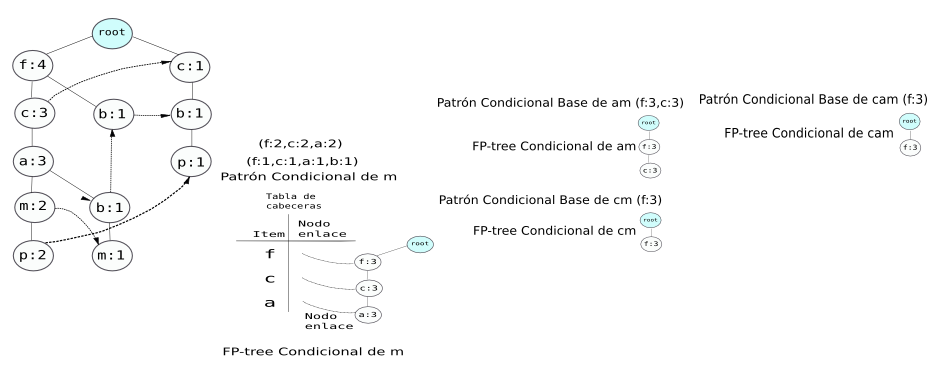
\includegraphics[width=1\textwidth]{images/fpcondicional.png}
   \caption{FP-tree condicional para $m$}
   \label{fpcondicional}
\end{figure}

En la siguiente tabla se muestran los Patrones Condicionales Base y los FP-trees generados.

\begin{table}[h]
\caption{Patrones Condicionales Base y FP-trees Condicionales}
\end{table}
\begin{center}
\begin{tabular}{|p{10mm}|p{76mm}|p{42mm}|}\hline
\textbf{Item} & \textbf{Patr\'on Condicional Base} & \textbf{FP-tree condicional}\\ \hline
$p$ & $\{(f:2,c:2,a:2,m:2),(c:1,b:1)\}$			& $\{(c:3)\}|p$\\ \hline
$m$ & $\{(f:2,c:2,a:2),(f:1,c:1,a:1,b:1)\}$		& $\{(f:3,c:3,a:3)\}|m$\\ \hline
$b$ & $\{(f:1,c:1,a:1),(f:1),(c:1)\}$			& $\phi$\\ \hline
$a$ & $\{(f:3,c:3)\}$					& $\{(f:3,c:3)\}|a$\\ \hline
$c$ & $\{(f:3)\}$					& $\{(f:3)\}|c$\\ \hline
$f$ & $\phi$						& $\phi$\\ \hline
\end{tabular}
\end{center}

Como se dijo anteriormente los Patrones Frecuentes se obtienen a partir de las combinaciones de cada uno de los
items con sus Patrones Condicionales Base. Por ejemplo para $m$, sus Patrones Frecuentes 
$\{(m:3),(am:3),(cm:3),(fm:3),(cam:3),(fam:3),(fcam:3),(fcm:3)\}$, son obtenidos de combinar a $m$ con cada uno
de sus Patrones Condicionales Base $\{(f:2,c:2,a:2),(f:1,c:1,a:1,b:1)\}$.

\subsection{EquipAsso}

\begin{enumerate}
\item Nuevos Operadores Del Algebra Relacional Para Asociaci\'on.
\begin{enumerate}
\item Operador Associator ($\alpha$)\\
Associator($\alpha$) es un operador algebraico unario que al contrario del operador Selecci\'on o 
Restricci\'on ($\sigma$), aumenta la cardinalidad o el tama\~no de una relaci\'on ya que genera a partir de cada
tupla de una relaci\'on, todas las posibles combinaciones de los valores de sus atributos, como tuplas de una
nueva relaci\'on conservando el mismo esquema. Por esta raz\'on esta operaci\'on, debe ser posterior a la 
mayor\'ia de operaciones en el proceso de optimizaci\'on de una consulta.\\ \\
Su sintaxis es la siguiente:\\
\begin{center}$\alpha_{tam_inicial, tam_final}$(R)\end{center}
El operador Associator genera, por cada tupla de la relaci\'on R, todos sus posibles subconjuntos (itemsets)
de diferente tama\~no. Associator toma cada tupla t de R y dos par\'ametros: $\<tam\_inicial\>$ y 
$\<tam_final\>$ como entrada, y retorna, por cada tupla t, las diferentes combinaciones de atributos
$X_{i}$, de tama\~no $\<tam\_inicial\>$ hasta tama\~no $\<tam\_final\>$, como tuplas en una nueva
relaci\'on. El orden de los atributos en el esquema de R determina los atributos en los subconjuntos con valores,
el resto se hacen nulos. El tama\~no m\'aximo de un itemset y por consiguiente el tama\~no final m\'aximo
$(\<tam\_final\>)$ que se puede tomar como entrada es el correspondiente al valor del grado de la relaci\'on.\\
Formalmente, sea $A=\{A_{1},...,A_{n}\}$ el conjunto de atributos de la relaci\'on R de grado n y cardinalidad m,
IS y ES el tama\~no inicial y final respectivamente de los subconjuntos a obtener. El operador $\alpha$ aplicado
a  R.

\begin{center}
$\alpha_{IS,ES}(R)=\{ \cup_{all}\ \ X_{i}\ \ |\ \ X_{i} \subseteq t_{i},\ \ t_{i} \in R, \forall_{i}
\forall_{k}(X_{i}=
\< v_{i}(A_{1}),v_{i}(A_{2}),null,...,v_{i}(A_{k}),null\>,v_{i}(A_{k})\< \> null),(i=(2^{n}-1)*m), (k=IS,...,ES),
\ \ A_{1}\< A_{2}\< ...A_{k},\ \ IS=1,ES=n\}$
\end{center}

produce una nueva relaci\'on cuyo esquema R(A) es el mismo de R de grado n y cardinalidad $m'=(2^{n}-1)*m$ y cuya
extensi\'on r(A) est\'a formada por todos los subconjuntos $X_{i}$ generados a partir de todas las combinaciones
posibles de los valores no nulos $v_{i}(A_{k})$ de los atributos de cada tupla $t_{i}$ de R. En cada tupla $X_{i}$
\'unicamente un grupo de atributos mayor o igual que IS y menor o igual que ES tienen valores, los dem\'as
atributos se hacen nulos.\\ \\
\textbf{Ejemplo 1}. Sea la relaci\'on R(A,B,C,D):

\begin{center}
\begin{tabular}{|c|c|c|c|}\hline
\textbf{A} & \textbf{B} & \textbf{C} & \textbf{D}\\ \hline
a1 & b1 & c1 & d1\\ \hline
a1 & b2 & c1 & d2\\ \hline
\end{tabular}
\end{center}

El resultado de $R1=\alpha_{2,4}(R)$, se puede observar en la figura \ref{r1}.

\item Operador Equikeep ($\chi$)\\
Equikeep ($\chi$) es un operador unario que restringe los valores de los atributos de cada una de las tuplas de la
relaci\'on R a \'unicamente los valores de los atributos que satisfacen una expresi\'on l\'ogica.\\ \\
Su sintaxis es la siguiente:\\ \\
$\chi_{expresion\_ logica}(R)$

\begin{table}[ht]
\caption{Resultado de $R1=\alpha_{2,4}(R)$}
\label{r1}
\end{table}
\begin{center}
\begin{tabular}{|c|c|c|c|}\hline
\textbf{A}    & \textbf{B}    & \textbf{C}    & \textbf{D}\\ \hline
a1   & b1   & null & null\\ \hline
a1   & null & c1   & null\\ \hline
a1   & null & null & d1\\ \hline
null & b1   & c1   & null\\ \hline
null & b1   & null & d1\\ \hline
null & null & c1   & d1\\ \hline
a1   & b1   & c1   & null\\ \hline
a1   & b1   & null & d1\\ \hline
a1   & null & c1   & d1\\ \hline
null & b1   & c1   & d1\\ \hline
a1   & b1   & c1   & d1\\ \hline
a1   & b2   & null & null\\ \hline
a1   & null & c1   & null\\ \hline
a1   & null & null & d2\\ \hline
null & b2   & c1   & null\\ \hline
null & b2   & null & d2\\ \hline
null & null & c1   & d2\\ \hline
a1   & b2   & c1   & null\\ \hline
a1   & b2   & null & d2\\ \hline
a1   & null & c1   & d2\\ \hline
null & b2   & c1   & d2\\ \hline
a1   & b2   & c1   & d2\\ \hline
\end{tabular}
\end{center}

El operador EquiKeep restringe los valores de los atributos de cada una de las tuplas de la relaci\'on R a
\'unicamente los valores de los atributos que satisfacen una expresi\'on l\'ogica $\<expr\_log\>$, la cual esta
formada por un conjunto de cl\'ausulas de la forma Atributo=Valor, y operaciones l\'ogicas AND, OR y NOT.
En cada tupla, los valores de los atributos que no cumplen la condici\'on $\<expr\_log\>$ se hacen nulos.
EquiKeep elimina las tuplas vac\'ias, i.e. las tuplas con todos los valores de sus atributos nulos.\\ \\
Formalmente, sea $A={A_{1},...,A_{n}}$ el conjunto de atributos de la relaci\'on R de esquema R(A), de grado n y
cardinalidad m. Sea p una expresi\'on l\'ogica integrada por cl\'ausulas de la forma $A_{i}=const$ unidas por los
operadores booleanos AND (\^{}), OR $(v)$, NOT $(\neg)$. El operador $\chi$ aplicado a la relaci\'on R con la
expresi\'on l\'ogica p:
\begin{center}
$\chi_{p}(R)=\{t_{i}(A)|\forall_{i}\forall_{j}(p(v_{i}(A_{j}))=v_{i}(A_{j})\ \ si\ \ p=true\ \ y\ \
p(v_{i}(A_{j}))=null\ \ si\ \ p=false),i=1...m',j=1...n,\ \ m'\leq m \}$
\end{center}
produce una relaci\'on de igual esquema R(A) de grado n y cardinalidad $m'$, donde $m'\leq m$. En su extensi\'on,
cada n-tupla $t_{i}$, esta formada por los valores de los atributos de R, $v_{i}(A_{j})$, que cumplan la
expresi\'on l\'ogica p, es decir $p(v_{i}(Y_{j}))$ es verdadero, y por valores nulos si $p(v_{i}(Y_{j}))$ es
falso.\\ \\
\textbf{Ejemplo 2}. Sea la relaci\'on R(A,B,C,D) y la operaci\'on $\chi_{A=a1 \lor B=b1 \lor C=c2 \lor
D=d1}(R)$:

\begin{center}
\begin{tabular}{|c|c|c|c|}\hline
\textbf{A} & \textbf{B} & \textbf{C} & \textbf{D}\\ \hline
a1 & b1 & c1 & d1\\ \hline
a1 & b2 & c1 & d2\\ \hline
a2 & b2 & c2 & d2\\ \hline
a2 & b1 & c1 & d1\\ \hline
a2 & b2 & c1 & d2\\ \hline
a1 & b2 & c2 & d1\\ \hline
\end{tabular}
\end{center}

El resultado de esta operaci\'on es la siguiente:

\begin{center}
\begin{tabular}{|c|c|c|c|}\hline
\textbf{A} & \textbf{B} & \textbf{C} & \textbf{D}\\ \hline
a1   & b1   & null & d1\\ \hline
a1   & null & null & null\\ \hline
null & null & c2   & null\\ \hline
null & b1   & null & d1\\ \hline
null & null & null & null\\ \hline
a1   & null & c2   & d1\\ \hline
\end{tabular}
\end{center}

\end{enumerate}
\item Algoritmo EquipAsso\\
El primer paso del algoritmo simplemente cuenta el n\'umero de ocurrencias de cada item para determinar los
1-itemsets frecuentes. En el subsiguiente paso, con el operador EquiKeep se extraen de todas las
transacciones los itemsets frecuentes tama\~no 1 haciendo nulos el resto de valores. Luego se aplica el operador
Associator desde $I_{s}=2$ hasta el grado n. A continuaci\'on se muestra el algoritmo Equipasso:

\begin{footnotesize}
$L1=\{1-itemsets\ \ frecuentes\};$\\
forall $transacciones\ \ t\in D$ do begin\\
\indent $R=\chi_{L1}(D)$\\
\indent $K=2$\\
\indent $g=grado(R)$\\
\indent $R'=\alpha_{k,g}(R)$\\
end\\
$L_{k}=\{count(R')|c.count\geq minsup\}$\\
Respuesta $=\cup L_{k};$
\end{footnotesize}
\end{enumerate}

%%%%%%%%%%%%%%%%%%%%%%%%%%%%%%%%%%%%%%%%%% Estado del arte %%%%%%%%%%%%%%%%%%%%%%%%%%%%%%%%%%%%%%%%%%%%%%%%%%
\section{Estado del Arte}
En el desarrollo de nuestro trabajo de grado realizamos un estudio de herramientas de miner\'ia de datos
elaboradas por otras universidades y centros de investigaci\'on que nos permitieron ver el estado actual de este
tipo de aplicaciones. A continuaci\'on se describen las herramientas estudiadas.

\subsection{WEKA - Waikato Environment for Knowledge Analysis}
WEKA es una herramienta libre de miner\'ia de Datos realizada en el departamento de Ciencias de la Computaci\'on
de la Universidad de Waikato en Hamilton, Nueva Zelanda.  Los principales gestores de este proyecto son Ian H.
Waitten y Eibe Frank autores del libro Data Mining: Practical Machine Learning Tools and Techniques with Java
Implementations \cite{37} cuyo octavo cap\'itulo sirve como tutorial de Weka y es libremente distribuido junto con
el ejecutable y el c\'odigo fuente.  Las ultimas versiones estables de Weka pueden ser descargadas de la p\'agina
oficial del Proyecto \cite{38}.\\

La implementaci\'on de la herramienta fue hecha bajo la plataforma Java utilizando la versi\'on 1.4.2 de su
m\'aquina virtual.  Al ser desarrollada en Java, Weka posee todas las caracter\'isticas de una herramienta
orientada a objetos con la ventaja de ser multiplataforma, la ultima versi\'on (3.4) ha sido evaluada bajo
ambientes GNU/Linux, Macintosh y Windows siguiendo una arquitectura Cliente/Servidor lo que permite ejecutar
ciertas tareas de mane\-ra distribuida.\\

La conexi\'on a la fuente de datos puede hacerse directamente hacia un archivo plano, considerando varios formatos
como C4.5 y CVS aunque el formato oficial es el ARFF que se explica m\'as adelante, o a trav\'es de un driver JDBC
hacia diferentes Sistemas Gestores de Bases de Datos(SGBD).\\

Entre las principales caracter\'isticas de Weka esta su modularidad la cual se fundamenta en un estricto y
estandarizado formato de entrada de datos que denominan ARFF (Atributte - Relation File Format), a partir de este
tipo de archivo todos los algoritmos de miner\'ia implementados en Weka son trabajados.  Nuevas implementaciones y
adiciones deben ajustarse a este formato.\\

El formato ARFF consiste en una archivo sencillo de texto que funciona a partir de etiquetas, similar a XML, y
que debe cumplir con dos secciones: una cabecera y un conjunto de datos.  La cabecera contiene las etiquetas del
nombre de la relaci\'on (@relation) y los atributos (@atributte), que describen los tipos y el orden de los
datos. La secci\'on datos (@data) en un archivo ARFF contiene todos los datos del conjunto que se quiere evaluar
separados por comas y en el mismo orden en el que aparecen en la secci\'on de atributos \cite{arff}.\\

La conexi\'on al SGBD se hace en primera instancia a trav\'es de una interfaz gr\'afica de usuario construyendo
una sentencia SQL siguiendo un modelo relacional pero a partir de construida la tabla a minar se trabaja en
adelante fuera de l\'inea a trav\'es de flujos (streams) que se comunican con archivos en disco duro.\\

WEKA cubre gran parte del proceso de Descubrimiento de Conocimiento, las caracter\'isticas especificas de
miner\'ia de datos que se pueden ver son pre-procesamiento y an\'alisis de datos, clasificaci\'on, clustering,
asociaci\'on y visualizaci\'on de resultados.\\

WEKA posee una rica colecci\'on de algoritmos que soportan el proceso de miner\'ia que aplican diversas
metodolog\'ias como arboles de decisi\'on, conjuntos difusos, reglas de inducci\'on, m\'etodos estad\'isticos y
redes bayesianas.\\

Por poseer diferentes modos de interfaces gr\'aficas, WEKA se puede considerar una herramienta orientada al
usuario aunque cabe aclarar que exige un buen dominio de conceptos de miner\'ia de datos y del objeto de
an\'alisis.  Muchas tareas se encuentran soportadas aunque no del todo automatizadas por lo que el proceso de
descubrimiento debe ser guiado a\'un por un analista.\\

Un an\'alisis completo de las caracter\'isticas de WEKA con respecto a otras aplicaciones presentes en el mercado
se puede encontrar en \cite{10}.

\subsection{ADaM - Algorithm Development and Mining System}
El proyecto ADaM es desarrollado por el Centro de Sistemas y Tecnolog\'ias de la Informaci\'on de la Universidad
de Alabama en Huntsville, Estados Unidos.  Este sistema es usado principalmente para aplicar t\'ecnicas de
miner\'ia a datos cient\'ificos obtenidos de sensores remotos \cite{adam}.\\

ADaM es un conjunto de herramientas de miner\'ia y procesamiento de im\'agenes que consta de varios componentes
interoperables que pueden u\-sarse en conjunto para realizar aplicaciones en la soluci\'on de diversos
pro\-blemas. En la actualidad, ADaM (en su versi\'on 4.0.2) cubre cerca de 120 componentes \cite{adamComp} que
pueden ser configurados para crear procesos de mine\-r\'ia personalizados.  Nuevos componentes pueden f\'acilmente
integrarse a un sistema o proceso existente.\\

ADaM 4.0.2 provee soporte a trav\'es del uso de componentes aut\'onomos dentro de una arquitectura distribuida. 
Cada componente esta desarrollado en C, C++ u otra interfaz de programaci\'on de aplicaciones y entrega un
ejecutable a modo de script donde cada componente recibe sus par\'ametros a trav\'es de l\'inea de comandos y
arroja los resultados en ficheros que pueden ser utilizados a su vez por otros componentes ADaM.  Eventualmente
se ofrece Servicios Web de algunos componentes por lo que se puede acceder a ellos a trav\'es de la Web.\\

Lastimosamente el acceso a fuentes de datos es limitada no ofreciendo conexi\'on directa hacia un sistema gestor
de bases de datos. ADaM trabaja generalmente con ficheros ARFF \cite{arff} que son generados por sus
componentes.\\

Dentro de las herramientas ofrecidas por ADaM encontramos soporte al preprocesamiento de datos y de im\'agenes,
clasificaci\'on, clustering y asociaci\'on.  La visualizaci\'on y an\'alisis de resultados se deja para ser 
implementado por el sistema que invoca a los componentes. ADaM 4.0.2 ofrece un amplio conjunto de herramienta que
implementa diversos metodolog\'ias dentro del \'area del descubrimiento de conocimiento.  Existen m\'odulos que
implementan \'arboles de decisi\'on, reglas de asociaci\'on, m\'etodos estad\'isticos, algoritmos gen\'eticos y
redes bayesianas.\\

ADaM 4.0.2 no soporta una interfaz gr\'afica de usuario, se limita a ofrecer un conjunto de herramientas para ser
utilizadas en la construcci\'on de sistemas que cubran diferentes \'ambitos.  Por tal motivo, es necesario un buen
conocimiento de los conceptos de miner\'ia de datos, a parte de fundamentos en el an\'alisis y procesamiento de
im\'agenes.  No obstante, ADaM ofrece un muy buen soporte a sistemas donde se busque descubrimiento de
conocimiento, un ejemplo de la implementaci\'on de ADaM puede verse en \cite{adamImpl} donde se utilizan
componentes ADaM en el an\'alisis e interpretaci\'on de im\'agenes satelitales de ciclones para estimar la
m\'axima velocidad de los vientos.

\subsection{Orange - Data Mining Fruitful and Fun}
Constru\'ido en el Labor\'atorio de Inteligencia Artif\'icial de la F\'acultad de Computaci\'on y Ciencias de la
Informaci\'on de la Universidad de Liubliana, en Eslovenia y ya que fu\'e liberado bajo la Licencia P\'ublica
General (GPL) puede ser descargado desde su sitio oficial \cite{oran}.\\

Orange \cite{oranwp} en su n\'ucleo es una librer\'ia de objetos C++ y rutinas que incluyen entre otros,
algoritmos estandar y no estandar de Miner\'ia de Datos y Aprendizaje Maquinal, adem\'as de rutinas para la
entrada y manipulaci\'on de datos. Orange provee un ambiente para que el usuario final pueda acceder a la
herramienta a trav\'es de scripts hechos en Python y que se encuentran un nivel por encima del n\'ucleo en  C++.
Entonces el usuario puede incorporar nuevos algoritmos o utilizar c\'odigo ya elaborado y que le permiten cargar,
limpiar y minar datos, as\'i como tambi\'en imprimir \'arboles de desici\'on y reglas de asociaci\'on.\\

Otra caracter\'istica de Orange es la inclusi\'on de un conjunto de Widgets gr\'aficos que usan m\'etodos y
m\'odulos del n\'ucleo central (C++) brindando una intef\'az agradable e intuitiva al usuario.\\

Los Widgets de la interfaz gr\'afica y los m\'odulos en Python incluyen tareas de Miner\'ia de Datos desde 
preprocesamiento hasta modelamiento y evaluaci\'on. Entre otras funciones estos componentes poseen t\'ecnicas
para:

\begin{description}
\item [Entrada de datos] Orange proporciona soporte para varios formatos popu\-lares de datos. Como por ejemplo:
	\begin{description}
	\item  [.tab] Formato nativo de Orange. La primera l\'inea tiene los nombres de los atributos, la segunda
	l\'inea dice cual es el tipo de datos de cada columna (discreto o continuo) y en adelante se encuentran
	los datos separados a trav\'es de tabuladores.
	\item [.c45] Estos archivos est\'an compuestos por dos archivos uno con extenci\'on .names que tiene los
	nombres de las columnas separados por comas y otro .data con los datos separados tambi\'en con comas.
	\end{description}
	
\item [Manipulaci\'on de datos y preprocesamiento] Entre las tareas que Oran\-ge incluye en este apartado tenemos
visualizaci\'on gr\'afica y estad\'istica de datos, procesamiento de filtros, discretizaci\'on y construcci\'on
de nuevos atributos entre otros m\'etodos.

\item [Miner\'ia de Datos y Aprendizaje M\'aquinal] Dentro de esta rama Oran\-ge incluye variedad de algoritmos
de asociaci\'on, clasificaci\'on, regresi\'on logistica, regresi\'on lineal, \'arboles de regresi\'on y
acercamientos basados en instancias (instance-based approaches).

\item [Contenedores] Para la calibraci\'on de la predicci\'on de probabilidades de modelos de clasificaci\'on.

\item [M\'etodos de evaluaci\'on] Que ayudan a medir la exactiud de un clasificador.
\end{description}

Podr\'ia catalogarse como una falencia el hecho de que Orange no incluya un modulo para la conexi\'on a un Sistema
Gestor de Bases de Datos, pero si se revisa bien la documentaci\'on de los modulos se encuentra que ha sido
desarrollado uno para la conexi\'on a MySQL (orngMySQL \cite{oransql}). El modulo provee una entrada a MySQL a
trav\'es de este modulo y de sencillos comandos en Python los datos de las tablas pueden transferidos desde y
hacia MySQL. As\'i mismo programadores independientes han desarrollado varios modulos entre los que se destaca
uno para algoritmos de Inteligencia Artificial.\\

Dentro de las herramientas de Miner\'ia de Datos, Orange podr\'ia catalogar\-se como una Herramienta Gen\'erica
Multitarea. Estas herramientas realizan una variedad de tareas de descubrimiento, t\'ipicamente combinando
clasificaci\'on, asociaci\'on , visualizaci\'on, clustering, entre otros. Soportan diferentes etapas del proceso
de DCBD.  El usuario final de estas herramientas  es un analista quien entiende la manipulaci\'on de los datos.\\

Orange funciona en varias plataformas como Linux, Mac y Windows y desde su sitio web \cite{oran} se puede
descargar toda la documentaci\'on disponible para su instalaci\'on. Al instalar Orange el usuario puede acceder a
una completa informaci\'on de la herramienta, as\'i como a pr\'acticos tutoriales y manuales que permiten
familiarizarse con la misma. Su sitio web \cite{oran} incluye tutoriales b\'asicos sobre Python y Orange,
manuales para desarrolladores m\'as avanzados y adem\'as tener acceso a los foros de Orange en donde se despejan
todos los interrogantes sobre esta herramienta.\\

En si Orange esta hecho para usuarios experimentados e investigadores en aprendizaje maquinal con la ventaja de
que el software fue liberado con licencia GPL, por tanto cualquier persona es libre de desarrollar y probar sus
propios algoritmos reusando tanto c\'odigo como sea posible.

\subsection{TANAGRA - A Free Software for Research and Academic Purposes}

TANAGRA \cite{rico} es software de Miner\'ia de Datos con pr\'opositos ac\'ademicos e investigativos,
desarrollado por Ricco Rakotomalala, miembro del Equipo de Investigaci\'on en Ingenier\'ia del Conocimiento (ERIC
- Equipe de Recherche en Ing\'enierie des Connaissances \cite{eric}) de la Universidad de Lyon, Francia. Conjuga
varios m\'etodos de Miner\'ia de Datos como an\'alisis exploratorio de datos, aprendizaje estad\'istico y
aprendizaje maquinal.\\

Este proyecto es el sucesor de SIPINA, el cu\'al implementa varios algoritmos de aprendizaje supervisado,
especialmente la construcci\'on visual de \'arboles de desici\'on. TANAGRA es m\'as potente, contiene adem\'as de
algunos paradigmas supervisados, clustering, an\'alisis factorial, estad\'istica param\'etrica y
no-param\'etrica, reglas de asociaci\'on, selecci\'on de caracter\'isticas y cons\-trucci\'on de algoritmos.\\

TANAGRA es un proyecto open source, as\'i que cualquier investigador puede acceder al c\'odigo fuente y a\~nadir
sus propios algoritmos, en cuanto este de acuerdo con la licencia de distribuci\'on.\\

El principal pr\'oposito de TANAGRA es proponer a los investigadores y estudiantes una arquitectura de software
para Miner\'ia de Datos que permita el an\'alisis de datos tanto reales como sint\'eticos.\\

El segundo pr\'oposito de TANAGRA es proponer a los investigadores una arquitectura que les permita a\~nadir sus
propios algoritmos y m\'etodos, para as\'i comparar sus rendimientos. TANAGRA es m\'as una plataforma
experimental, que permite ir a lo esencial y obviarse la programaci\'on del manejo de los datos.\\

El tercero y \'ultimo pr\'oposito va dirigido a desarrolladores novatos y consiste en difundir una metodolog\'ia
para construir este tipo de software con la ventaja de tener acceso al c\'odigo fuente, de esta forma un
desarrollador puede ver como ha sido construido el software, cuales son los problemas a evadir, cuales son los
principales pasos del proyecto y que herramientas y librer\'ias usar.\\

Lo que no incluye TANAGRA es lo que constituye la fuerza del software comercial en el campo de la Miner\'ia de
Datos: Grandes fuentes de datos, acceso directo a bodegas y bases de datos (Data Warehouses y Data Bases) as\'i
como la aplicaci\'on de data cleaning.\\

Para realizar trabajos de Miner\'ia de Datos con Tanagra, se deben crear esquemas y diagramas de flujo y utilizar
sus diferentes componentes que van desde la visualizaci\'on de datos, estad\'isticas, construcci\'on y
selecci\'on de ins\-tancias, regresi\'on y asociaci\'on entre otros.\\

El formato del conjunto de datos de Tanagra es un archivo plano (.txt) separado por tabulaciones, en la primera
l\'inea tiene un encabezado con el nombre de los atributos y de la clase, a continuaci\'on vienen los datos con
el mismo formato de separaci\'on con tabuladores. Tanagra tambi\'en acepta conjuntos de datos generados en Excel
y uno de los estandares en Miner\'ia de Datos, el formato de WEKA (archivos .arff). Tanagra permite cargar un
solo conjunto de datos.\\

A medida que se trabaja con TANAGRA y se van generando reportes de resultados, existe la posibilidad de
guardarlos en formato HTML.\\

La paleta de componentes de Tanagra tiene implementaciones de tareas de Miner\'ia de Datos que van desde
preprocesamiento hasta modelamiento y evaluaci\'on. Entre otras TANAGRA permite usar t\'ecnicas para:

\begin{description}
\item [Entrada de datos] Con soporte para varios formatos populares de datos.
\item [Manipulaci\'on de datos y preprocesamiento] Como muestreo, filtrado, discretizaci\'on y construcci\'on de nuevos atributos entre otros m\'etodos.
\item [Construcci\'on de Modelos] M\'etodos para la construcci\'on de modelos de clasificaci\'on, que incluyen \'arboles de clasificaci\'on, clasificadores Naive-Bayes y regresi\'on log\'istica.
\item [M\'etodos de regresi\'on] Como regresi\'on multiple lineal.
\item [M\'etodos de evaluaci\'on] Utilizados para medir la exactitud de un clasificador.
\end{description}

Al ser TANAGRA un proyecto Open Source es facilmente descargable desde su sitio web \cite{tana}, el cual contiene
tutoriales, referencias y conjuntos de datos.

\subsection{AlphaMiner}

AlphaMiner es desarrollado por el E-Business Technology Institute (ETI) de la Universidad de Hong Kong \cite{eti}
bajo el apoyo del Fondo para la Innovaci\'on y la Tecnolog\'ia (ITF) \cite{itf} del Gobierno de la Regi\'on
Especial Admi\-nistrativa de Hong Kong (HKSAR).\\

AlphaMiner es un sistema de Miner\'ia de Datos, Open Source, desarro\-llado en java de prop\'osito general pero
m\'as enfocado al ambiente  empresa\-rial. Implementa algoritmos de asociaci\'on, clasificaci\'on, clustering y
regresi\'on log\'istica. Posee una gama amplia de funcionalidad para el usuario, al realizar cualquier proceso
minero dando la posibilidad al usuario de escoger los pasos del proceso KDD que m\'as se ajusten a sus
necesidades, por medio de nodos que el analista integra a un \'arbol KDD siguiendo la metodolog\'ia Drag \& Drop. 
Es por eso que el proceso KDD en AlphaMiner no sigue un orden estructurado, sino que sigue la secuencia  brindada
por el prop\'osito u objetivo  del analista, ademas brinda la visualicion estad\'istica de distintas maneras, 
permitiendo un analisis m\'as preciso por parte del analista.\\

El principal objetivo de AlphaMiner es la inteligencia Comercial Econ\'omica o Inteligencia de Negocios (BI -
Business Inteligence) es uno de los  medios m\'as importantes para que las compa\~n\'ias tomen las decisiones
comerciales m\'as acertadas. Las soluciones de BI son costosas y s\'olo empresas grandes pueden permitirse el
lujo de tenerlas. Por tanto las compa\~n\'ias peque\~nas tienen una gran desventaja. AlphaMiner proporciona las
tecnolog\'ias de BI de forma econ\'omica para dichas empresas para que den soporte a sus decisiones en el
ambiente de negocio cambiante r\'apido.\\
   
AlphaMiner tiene dos componentes principales:
\begin{enumerate}
\item Una base de conocimiento.
\item Un \'arbol KDD, que permite integrar nodos artefacto que proporcionan varias funciones para crear, revisar,
anular, interpretar y argumentar los distintos an\'alisis de datos
\end{enumerate}

AlphaMiner implementa los siguientes pasos del proceso KDD:
\begin{enumerate}
\item Acceso de diferentes formas a las fuentes datos.
\item Exploraci\'on de datos de diferentes maneras.
\item Preparaci\'on de datos.
\item Vinculaci\'on de los distintos modelos mineros.
\item An\'alisis a partir de los  modelos.
\item Despliegue de modelos al ambiente  empresarial.   
\end{enumerate}

La caracter\'istica m\'as importante de AlphaMiner, es su capacidad para almacenar los datos despu\'es del
n\'ucleo minero en una base de conocimiento, que puede ser reutilizada. Esta funci\'on aumenta su utilidad
significativamente, y  brinda un gran apoyo log\'istico al nivel estrat\'egico de una empresa. Aventajando
cualquier sistema tradicional de manipulaci\'on de datos. AlphaMiner proporciona una funcionalidad adicional para
construir los modelos de Miner\'ia de Datos, conformando una sinergia entre los distintos algoritmos de
miner\'ia.\\

AlphaMiner se asemeja a Tariy en varias caracter\'isticas, por un lado el lenguaje de programaci\'on en el que
fue implementado es JAVA, por otro lado es Open Source, tiene conectividad JDBC a los distintos gestores de bases
de datos, adem\'as de conectividad con archivos de Excel. Otra semejanza es el tipo de formato que presenta para
el manejo de  tablas un\'ivaluadas en algoritmos de asociaci\'on, espec\'ificamente en bases de datos de
supermercados, ya que despu\'es de escoger los campos de dicha base de datos se la lleva a un formato de dos
columnas una para la correspondiente transacci\'on y otra para el \'item.

\subsection{YALE - Yet Another Learning Environment}

YALE \cite{yalew, yalep} es un ambiente para la realizaci\'on de experimentos de aprendizaje maquinal y Miner\'ia
de Datos.  A trav\'es de un gran n\'umero de operadores se pueden crear los experimentos, los cuales pueden ser
anidados arbitrariamente y cuya configuraci\'on es descrita a trav\'es de archivos XML que pueden ser
f\'acilmente creados por medio de una interfaz gr\'afica de usuario.  Las aplicaciones de YALE cubren tanto
investigaci\'on como tareas de Miner\'ia de Datos del mundo real.\\

Desde el a\~no 2001 YALE ha sido desarrollado en la Unidad de Inteligencia Artificial de la Universidad de
Dortmund \cite{dort} en conjunto con el Centro de Investigaci\'on Colaborativa en Inteligencia Computacional
(Sonderforschungsbereich 531).\\

El concepto de operador modular permite el dise\~no de cadenas complejas de operadores anidados para el
desarrollo de un gran n\'umero de problemas de aprendizaje. El manejo de los datos es transparente para los
operadores. Ellos no tienen nada que ver con el formato de datos o con las diferentes presentaciones de los
mismos. El kernel de Yale se hace a cargo de las transformaciones necesarias.  Yale es ampliamente usada por
investigadores y compa\~n\'ias de Miner\'ia de Datos.

\subsubsection{Modelando Procesos De Descubrimiento De Conocimiento Como Arboles De Operadores}

Los procesos de descubrimiento de conocimiento son vistos frecuentemente como invocaciones secuenciales de
m\'etodos simples.  Por ejemplo, des\-pu\'es de cargar datos, uno podr\'ia aplicar un paso de preprocesamiento
seguido de una invocaci\'on a un m\'etodo de clasificaci\'on.  El resultado en este caso es modelo aprendido,
el cual puede ser aplicado a datos nuevos o no revisados todav\'ia.  Una posible abstracci\'on de estos m\'etodos
simples es el concepto de operadores. Cada operador recibe su entrada, desempe\~na una determinada funci\'on y
entrega una salida. Desde ahi, el m\'etodo secuencial de invocaciones corresponde a una cadena de operadores. 
Aunque este modelo de cadena es suficiente para la realizaci\'on de muchas tareas b\'asicas de descubrimiento de
conocimiento,  estas cadenas planas son a menudo insuficientes para el mo\-delado de procesos de descubrimiento de
conocimiento m\'as complejas.\\

Una aproximaci\'on com\'un para la realizaci\'on del dise\~no de experimentos m\'as complejos es dise\~nar las
combinaciones de operadores como un gr\'afico direccionado.  Cada vertice del gr\'afico corresponde a un operdor
simple. Si dos operadores son conectados, la salida del primer operador ser\'a usada como entrada en el segundo
operador.  Por un lado, dise\~nar procesos de des\-cubrimiento de conocimiento con la ayuda de
gr\'aficosdireccionados es muy poderoso.  Por el otro lado, existe una desventaja principal: debido a la
p\'erdida de restricciones y la necesidad de ordenar topol\'ogicamente el dise\~no de experimentos es menudo poco
intuitivo y las validaciones autom\'aticas son dif\'iciles de hacer.\\

Yale ofrece un compromiso entre la simplicidad de cadenas de operadores y la potencia de los gr\'aficos
direccionados a trav\'es del modelamiento de procesos de descubrimiento de conocimiento por medio de \'arboles de
operadores. Al igual que los lenguajes de programaci\'on , el uso de \'arboles de operadores permite el uso de
conceptos como ciclos, condiciones, u otros esquemas de aplicaci\'on.  Las hojas en el \'arbol de operadores
corresponden a pasos senci\-llos en el proceso modelado como el aprendizaje de un modelo de predicci\'on \'o la
aplicaci\'on de un filtro de preprocesamiento. Los nodos interiores del \'arbol corresponden a m\'as complejos o
abstractos pasos en el proceso.  Este es a menudo necesario si los hijos deben ser aplicados varias veces como,
por ejemplo, los ciclos.  En general, los nodos de los operadores internos definen el flujo de datos a trav\'es
de sus hijos. La raiz del \'arbol corresponde al experimento completo.

\subsubsection{Qu\'e Puede Hacer YALE?}

YALE provee mas de 200 operadores incluyendo:

\begin{description}
\item [Algoritmos de aprendizaje maquinal] Un gran n\'umero de esquemas de aprendizaje para tareas de regresi\'on
y clasificaci\'on incluyendo M\'aquinas para el Soporte de Vectores (SVM), \'arboles de decisi\'on e inductores
de reglas, operadores Lazy, operadores Bayesianos y operadores Log\'isticos. Varios operadores para la miner\'ia
de reglas de asociaci\'on y Clustering son tambi\'en parte de YALE.  Adem\'as, se adicionaron varios esquemas de
Meta Aprendizaje.

\item [Operadores WEKA] Todos los esquemas de aprendizaje y evaluadores de atributos del ambiente de aprendizaje
WEKA tambi\'en est\'an disponibles y pueden ser usados como cualquier otro operador de YALE.

\end{description}
